\documentclass[12pt]{article}
% This first part of the file is called the PREAMBLE. It includes
% customizations and command definitions. The preamble is everything
% between \documentclass and \begin{document}.

\usepackage[margin=1in]{geometry}  % set the margins to 1in on all sides
\usepackage{graphicx}              % to include figures
\usepackage{amsmath}               % great math stuff
\usepackage{amsfonts}              % for blackboard bold, etc
\usepackage{amsthm}                % better theorem environments

\usepackage{rotating} % for sideway table
\usepackage{xcolor}
\usepackage{hyperref}
\hypersetup{
    colorlinks,
    linkcolor={red!50!black},
    citecolor={blue!50!black},
    urlcolor={blue!80!black}
}
\usepackage{cleveref}

\usepackage{array,tabularx}

\newenvironment{conditions*}
  {\par\vspace{\abovedisplayskip}\noindent
   \tabularx{\columnwidth}{>{$}l<{$} @{${}={}$} >{\raggedright\arraybackslash}X}}
  {\endtabularx\par\vspace{\belowdisplayskip}}
  
\usepackage{float}
\restylefloat{table}

% various theorems, numbered by section

\newtheorem{thm}{Theorem}[section]
\newtheorem{lem}[thm]{Lemma}
\newtheorem{prop}[thm]{Proposition}
\newtheorem{cor}[thm]{Corollary}
\newtheorem{conj}[thm]{Conjecture}

\DeclareMathOperator{\id}{id}

\newcommand{\bd}[1]{\mathbf{#1}}  % for bolding symbols
\newcommand{\RR}{\mathbb{R}}      % for Real numbers
\newcommand{\ZZ}{\mathbb{Z}}      % for Integers
\newcommand{\col}[1]{\left[\begin{matrix} #1 \end{matrix} \right]}
\newcommand{\comb}[2]{\binom{#1^2 + #2^2}{#1+#2}}

% bibliography
\usepackage{natbib}
\bibpunct{(}{)}{;}{a}{}{,} % no comma between author and year

\title{Paper title}
\author{Anh Le}


\begin{document}
\maketitle

\section{Puzzle: FDI does not lead to development}

One of the most universally recommended development strategy in the past three decades is the attraction of foreign direct investment (FDI). The policy is pushed by major international organizations.\footnote{http://www.imf.org/external/pubs/ft/fandd/1999/03/mallampa.htm, http://www.weforum.org/reports/foreign-direct-investment-key-driver-trade-growth-and-prosperity-case-multilateral-agreement} Within political science, much of the literature assumes that countries seek FDI because of its many benefits. The challenge is \textit{how} can countries attract FDI, not whether it wants to attract it \citep{Jensen2003, Li2003, Li2006, Ahlquist2006}. On surface, this belief seems supported by the fact that the amount of FDI has increased greatly in the past decades (\Cref{fig:globalfdi}). The FDI flow to developing countries has not only steadily increased but is also remarkably robust to global economic downturns.

\begin{figure}[!ht]
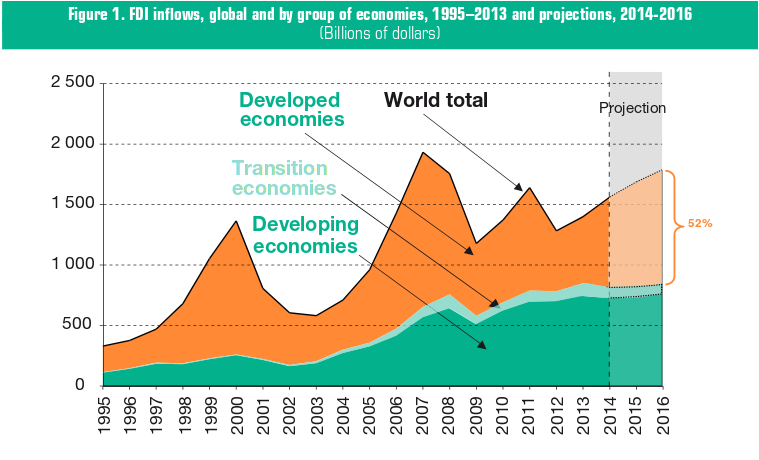
\includegraphics[width=\textwidth, height=\textheight,keepaspectratio]{../figure/global_fdi}
\caption{Source: World Investment Report, 2014}
\label{fig:globalfdi}
\end{figure}

The reason for this push is that FDI is hypothesized to bring various benefits to developing countries. FDI provides a source of capital which may generate employment (conditional on the fact that foreign firms may not put domestic firms to bankcruptcy, resulting in a net loss of employment). However, the most important promise of FDI is the spillover effect (in technology, human capital, and managerial practice) between the foreign firms and the domestic firms (this is assuming that the foreign firms are more advanced. This may not be true if foreign firms invest outside to seek cheap labor or to circumvent trade restriction). In endogenous growth theory, FDI is a major channel for technological innovation \citep{Findlay1978}.

Spillover can happened in different ways: competition (unless the incoming firm is granted monopoly status) similar to how arm's length trade put pressure on domestic firms to reduce inefficiency \citep{Glass2002}, imitation (both reverse engineering and copying managerial techniques, reverse engineering deserve government support) \citep{Wang1992}, human capital spillover of workers in foreign firms moving to domestic firms (Czech firms) \citep{Djankov2000}, technology transfer. Export demonstration, because exports often involve high fixed cost to set up a distribution and transport infrastructure, learn about foreign taste and regulatory framework. Domestic firms can learn from foreign firms about how to export, and exporting firms are more productive \citep{Aitken1997}.

However, there is no conclusive evidence of a consistent positive effect of FDI on growth and poverty reduction \citep{Guerra2009} (\Cref{fig:fdipoverty}).

Also, governments, both developed and developing have been provided massive incentives to FDI \citep{Telford2001}. For example, Ireland provided foreign investors with lower tax rate, lower land price, and cash grant for R\&D that do not need to be repaid. China also used a tax holiday (two years of no tax and three year of half the normal tax rate) in their special economic zones to attract more foreign firms. We see the same use of FDI incentives in Southeast Asia \citep{Fletcher2002}. The race to offer incentives to attract FDI rages on even among sub-national units. Defying central government's directive, Vietnam's provincial government offered extra-legal incentives to FDI \citep{Vu2007}

Investment incentives also does not work in promoting this link, because technology transfer is conditional \citep{Blomstrom2002}

TRIMS (trade related-investment measure) are not effective because it may lead to firms only bringing in bad technology due to local content requirement. So far there is little evidence, partly because the policy is hard to measure \citep{Greenaway1992}. The agreement on TRIMS also make this policy obsolete for trade-related investment (i.e. exporting firms).



\begin{figure}[!ht]
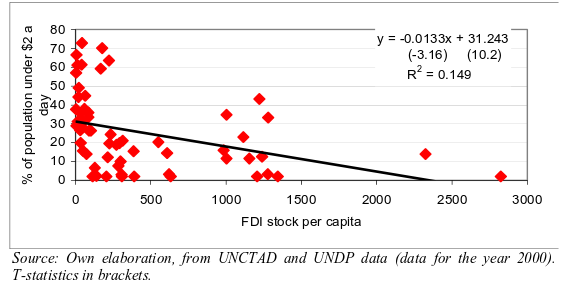
\includegraphics[width=\textwidth, height=\textheight,keepaspectratio]{../figure/fdi_poverty}
\caption{Relationship between FDI and poverty}
\label{fig:fdipoverty}
\end{figure}


\section{Puzzle 2: If absorptive capacity is important, why don't we see it more?}

Many works have been done on the importance of absorptive capacity. FDI is only growth enhancing when countries have cap -- a review \citep{Gorg2004}. Variation sub-nationally, China \citep{Fu2008}, crossnationally (absorptive capacity means financial and institutional--property rights--development)\citep{Durham2004}, Latin America (absorptive = educated workers) \citep{Willem2004}.

\section{Hypothesis: Rent seeking}

- corruption literature
- local central literature

Political decentralization increases bribery \citep{Fan2009}. Uncoordinated corruption, more tiers of governments, increase corruption.

Fiscal decentralization reduces corruption \citep{Guerra2009}

\section{Research design}

Hypothesis: In sectors / countries where there is a lot of corruption between the politicians and FDI, there will be less private sector development.

- corruption between the politicians and FDI: 

+ Vietnam case: 1) sectors with protection against FDI (group A) 

+ Vietnam + crossnational: 2) sectors with natural monopoly / high degree of profitability. Natural monopoly / profitability = access is more valuable means more incentive to bribe, small numbers of firms means easier coordination. (But why wouldn't the bureaucrat want to collude with the domestic firms instead? Perhaps because there are no big enough domestic firms. We can control for this by pre-FDI private sector)


- private sector development = measured on discretionary treatment measure (time deal with officials, officials' attitude, tax rate), not so much on infrastructure

\subsection{Crossnational}

Countries with a lot of corruption + a lot of FDI will see larger gap between the treatment of FDI and domestic firms.

Corruption alone is not enough. FDI alone is not enough.

What about corruption reducing FDI? Is there a sample of countries with high FDI and high corruption? (a graph would be neat)

INSERT GRAPH HERE


\subsection{Provincial leader vs central}

\citep{Malesky2008} Straight ahead on red -- central incentive is growth

\citep{Sheng2007} China's central government exert more control over provinces that has high FDI (through party organization channel)

\subsection{Sectoral}

\citep{Malesky2015} discusses how foreign firms in Group A restricted industries have to pay more bribes (telecommunications, radio and TV broadcasting, transportation, and distribution). We can use this as a measure of FDI corruption, especially since some of the restrictions applies to foreign firms only.


\subsection{Conjoint analysis}



- Selection bias (if a countries disriminated against FDI, then the surveyed firms are already more capable)


% http://zunia.org/sites/default/files/media/node-files/04/155466_04050041.pdf

Foreign firms often face fewer obstacles

Asia crowding in (SK, Thailand, pakistan), Latin America crowd out (crowdin or crowdout). Paper does not discuss the policy nor the motivation

Colombia, Mexico, Hong Kong, Indonesia, and Taiwan

Argentina, Brazil,Colombia, Korea, Malaysia, Thailand in Asia

Evidence is mixed across regions / countries DOES FOREIGN DIRECT INVESTMENT PROMOTE ECONOMIC GROWTH? EVIDENCE FROM EAST ASIA AND LATIN AMERICA 

in Latin America, high corruption = high FDI http://www.ccsenet.org/journal/index.php/jms/article/viewFile/32108/18686

http://www.nytimes.com/2012/04/22/business/at-wal-mart-in-mexico-a-bribe-inquiry-silenced.html?pagewanted=all (Walmart bribe in Mexico)

\clearpage
\bibliographystyle{chicago}
\bibliography{library}
\end{document}
